\pdfoutput=1
\documentclass[a4paper,pdflatex,ja=standard]{bxjsarticle}

% ---Setting about the geometry of the document----
% \usepackage{a4wide}
% \pagestyle{empty}

% ---Physics and Math Packages---
\usepackage{amssymb,amsfonts,amsthm,mathtools}
\usepackage{physics,braket,bm}

% ---underline---
\usepackage{ulem}

% --- surround the texts or equations
% \usepackage{fancybox,ascmac}

% ---settings of theorem environment---
% \usepackage{amsthm}
% \theoremstyle{definition}

% ---settings of proof environment---
% \renewcommand{\proofname}{\textbf{証明}}
% \renewcommand{\qedsymbol}{$\blacksquare$}

% ---Ignore the Warnings---
\usepackage{silence}
\WarningFilter{latexfont}{Some font shapes,Font shape}

% ---Insert the figure (If insert the `draft' at the option, the process becomes faster)---
% \usepackage{graphicx}
% \usepackage{subcaption}

% ----Add a link to a text---
\usepackage{url}
\usepackage{xcolor,hyperref}
\hypersetup{colorlinks=true,citecolor=orange,linkcolor=blue,urlcolor=magenta}
\usepackage{bxcjkjatype}

% ---Tikz---
% \usepackage{tikz,pgf,pgfplots,circuitikz}
% \pgfplotsset{compat=1.15}
% \usetikzlibrary{intersections,arrows.meta,angles,calc,3d,decorations.pathmorphing}

% ---Add the section number to the equation, figure, and table number---
\makeatletter
   \renewcommand{\theequation}{\thesection.\arabic{equation}}
   \@addtoreset{equation}{section}
   
  %  \renewcommand{\thefigure}{\thesection.\arabic{figure}}
  %  \@addtoreset{figure}{section}
   
   \renewcommand{\thetable}{\thesection.\arabic{table}}
   \@addtoreset{table}{section}
\makeatother

% ---enumerate---
% \renewcommand{\labelenumi}{$\arabic{enumi}.$}
% \renewcommand{\labelenumii}{$(\arabic{enumii})$}

% ---Index---
% \usepackage{makeidx}
% \makeindex 

% ---Fonts---
\renewcommand{\familydefault}{\sfdefault}

% ---Title---
\title{はじめに}
\author{ミヤネ}
\date{最終更新:\today}

\usepackage{comment}


\begin{document}

\maketitle

\tableofcontents
\clearpage

\begin{figure}[ht]
  \centering
  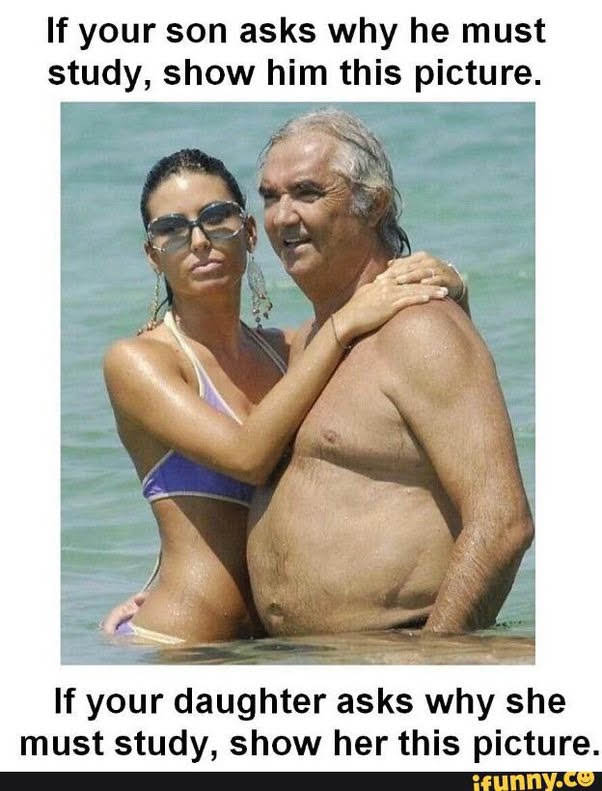
\includegraphics[keepaspectratio, scale=0.65]{fig/1690817582195.jpg}
  \caption{筆者の誕生日に友人が送ってくれた写真(面白かったので貼っちゃいました)}
\end{figure}


\clearpage

\section{このドライブについて}

\begin{itemize}
  \item 
  私が院試の勉強をしている際に解いた問題をまとめたものになります.少しづつ更新していきました.(このドキュメントも含めて)大半は勉強と並行しながら作成していったので,余裕のない雰囲気があるかと思います\footnote{
    試験を終えた人がああだこうだいうのは少し違うなと思いました(まあ,それでも有難いものかもしれません).
  }.少し見苦しいかもしれませんが,こういったのもアリだと思うので,あまりいじらないようにしておきます.

  \item 
  東大については,ネットに出回っている解答\footnote{
    \url{https://akinomyoga.github.io/ributsu-inshi-kakomon/}
  }との連携を意識して作りました.2009年より前の年度のものはその解答を,2010年度以降のは私のを参照していただければと思います.

  \item 
  早稲田と京大についても,一部だけですがTeXで解答を作成してみました.早稲田の解答については,ネットなどで出回っているものはありませんでした(もしかしたら,研究室によってはあるのかもしれません.少なからず,私が配属された研究室にはありませんでした).京大についてはこちらの解答\footnote{
    \url{https://kphysnote.amebaownd.com/pages/1848277/page_201804181651}
  }が公開されています.

  \item 
  この解答例が将来どうなるかは分かりませんが,私がインターネット上で公開することはないと思います.したがって,途切れたら終わりです.せっかく作ったのだから,これを見た人たちが加筆・修正したり,さらに新しい解答を作ったりして続いていけばなと思っています.
\end{itemize}


\section{解答について}

\begin{itemize}
  \item   
  参考文献は省略します.私自身が読んできた本はかなりスタンダードだと思います.例えば,
  \cite{sakurai,landau,kubo,goto,sunagawa_Q,sunagawa_E,tasaki_th,tasaki_stat1,tasaki_stat2}
  あたりでB1からB3の頃はよく勉強していました\footnote{
    そういえば,量子力学で有名な猪木・河合はレポートで参考にするくらいにしか読んでません.別に読んでなくても試験には困りませんでした.(「りろでん」や「久保統計」は院試のせいで読まれ続けてるという意見があるようですが,)有名な本はちゃんとそれなりの理由があって有名になっているので,読むと決めたらくだらない下心は捨てて真摯に読み込むべきだと私は思います(もちろん,それらを必ず読めというわけではないです).
  }.

  \item 
  大丈夫だとは思いますが,変な拡散はしないようにしてください.
  
  \item 
  計算ミスもあると思いますし,あまり自信がない解答もあります.そういったときは,周りと相談するなりして,解決していただければと思います.
  
  \item
  解答の細かさは,気分に依存しています.試験が近づくと解答が雑になっているような気がします.

  \item 
  pdfLaTeXで組んでしまっています.もし後から編集したい方で,困っている方がいたらすみません.
\end{itemize}



\section{大学別にコメント}

大学別に過去問を解いた感想を書いておこうと思います.


\subsection{早稲田大学}

基本的な問題が出題されますが,クセのある問題も多いです.物性のHSGW研の知人が言うには,「半分とれば,問答無用で受かる」と先生が漏らしていたそうです\footnote{
  恐らく,早稲田に関しては合否の権限が研究室にあると思われるので,研究室によって基準は変わってくると思います.(あまり大っぴらには言えませんが,許せないような酷いこともありました.外部を受験する人は,変な研究室に入らないよう,気をつけたほうがいいかもしれません.)
}.ちなみに,過去問があまり公開されてないため,あまり年数がありません.研究室を漁ってみると,何か出てくると思います.AB研にあったやつは,スキャンしてアップロードしておきました.(発見したときには時期が近かったので,解答は作ってません.)

\subsection{東京大学}

年度によってブレはありますが,誘導などがしっかりしているので解きやすいと思います.ただし,計算量は多いと感じました.「これ本当に計算するの?」というやつも普通に出してくる印象です.また,傾向が変わったようなので,実験は解かなくてもよいかもしれません.

また,来年度から英語が外部になるそうなので,受験を考えている人はTOEICなりを早いうちに受けておくと楽かもしれません.(ちなみに,早稲田もスコアの提出が必要です.)

\subsection{京都大学}

受験しないのでそんな本気で解いてるわけではないですが,掲載されている過去問が多いのと,バラエティーに富んでいたので練習でいくらかは解きました.全体的に難易度は抑え気味な感じがしますが\footnote{
  とはいえ,難しいのはもちろんあります.また,友人に見せてもらいましたが,昔の問題(2000年前後)はかなり鬼畜でした.
},なんといっても量が多いです.練習にはちょうどいいですが,受験するとなると大変そうです.

\section{その他}

\begin{itemize}
  \item 
  大学によって出題の形式は違いますが,逆に言えば違うのはそれぐらいしかないかと思います.もちろん,頻出の分野などはありますが,だからといってその大学の過去問を漁れば解けるようになるとは思えません\footnote{
    ただし,設問単位では複数回出題されているテーマはあるように思います.例えば,東大なら統計力学の状態数を求める問題とか,示量性を示す問題とか.(大学の方針なのか,それとも大学院入試の性質からそうなってしまうのかは分かりませんが.)
  }.受ける大学ばかりを解くのではなく,受験校以外の大学の問題を解いて,知見を広めるのも有効な対策だと思います(が,私はそんなに実行できたわけではありません...).

  \item 
  私は4月に入る直前くらいから,少しずつ問題を解いていました.ここらへんは人によって考え方は異なるかと思いますが,結局のところ,いつから対策を始めるのかについては,個々人の環境\footnote{
    研究室のdutyや単位取得状況,アルバイトなど.
  }
  ,学力\footnote{
    こればっかりは試験なので,ちゃんと身につけなければなりません.
  },プライド\footnote{
    受験勉強をしている間はやはりadvancedな勉強をする時間は削られてしまいます.私は研究室の文献紹介や超弦の講義を聴講したりして勉強した気にしていました.私もそうでしたが,この点は少しは気になるかと思います.ですが,こんなことを気にするほうが不健康なので,割り切るしかないんだと思います.
  }との相談になるかと思います.(私みたいに)ペーパーテストが苦手という自覚があるなら,少しずつ演習してみるのが良いかと思います.

  \item 
  ちなみに,ファイルや解答に書いてある年数は「入学する年」であり,「実施された年」ではないことに気をつけてください.例えば,「令和4年度」と書いてある試験は「令和4年度に入学する人を選別する」という意味なので,実施されているのは令和3年ということになります\footnote{
    つまり,令和2年 or 2021年の入試はありません.コロナでオンラインだったので.学部入試のときは,入学する年と実施した年が同じだったのであまり気にはなんなかったのですが,たぶん一般にこのように名前をつける慣習なんでしょう.
  }.

  \item
  計算ミスなどは潰しましょう.基本的な問題には部分点がないような気がしています.
  
  \item 
  また,困ったら手当たり次第に思いつく式 or 問題文にある式に代入してみるといいかもしれません.当然,論理とかを大事にして答えるのも大事ですが,そういったやり方でもそれっぽい答えがでることが多々あります.(物理の研究もそんなものかもしれません(笑))

  \item 
  時間制限は確かにあるのですが,計算力以上に知識が要求されている気がします.私は「計算が間に合わなかった」とか「時間あったら思いついた」といったことをあまり感じませんでした.

  \item 
  これは試験に限ったことではないですが,ある程度の結果の暗記は非常に有効だと思います.例えば「物質の境界面で電場$\bm{E}$と磁場$\bm{H}$は接線方向が等しい」といった事実はもちろん,「固体中の原子が調和振動していると近似すれば,比熱は低温では$T^3$に比例して,高温では一定」というような計算事実もある程度言えると物理に強くなれると思います\footnote{
    研究室に配属されて感じたことなのですが,先生やポスドクの人たちはこういったことの知識量がすごかったです(もちろん,根拠もすぐに言える感じでした).自分の専門分野について,ある程度進んだ知識を身に着けておくことは,アカデミアに残るためには大事なことなのでしょう.最初のうちは難しいと思いますが,慣れてきたら意識するべきだと思いました.
  }.

  \item 
  最初解いたときに「え,これを何も見ないで時間内に解くなんて無理なのでは?」と思いましたが,意外となんとかなりました.同じことを思う(思った)人がいるかもしれませんが,安心して勉強を頑張ってください.
\end{itemize}


\section{謝辞}

解答作成の際に色々な助言をくれたり,私の受験を応援してくださったみなさん,ありがとうございました.特に物理・応物の駒田君,福富君,林君は物理を教えてくれましたし,一緒に勉強してて楽しかったです.また,Wathematicaの岩波君,有原君,下田君は一緒にラーメンに行って励ましてくれました.とてもうれしかったです.



\begin{thebibliography}{99}
  \bibitem{sakurai} J.J. Sakurai, S.F. Tuan, \textit{Modern Quantum Mechanics.} Benjamin/Cummings Pub., 1985.
  \bibitem{landau} ランダウ=リフシッツ, 『力学』. 東京図書, 2022.
  \bibitem{kubo} 久保亮五, 『大学演習熱学・統計力学』. 裳華房, 1998.
  \bibitem{goto} 後藤憲一, 神吉健, 山本邦夫, 『詳解物理/応用数学演習』. 共立出版, 1979.
  \bibitem{sunagawa_Q} 砂川重信, 『量子力学』. 岩波書店, 1991.
  \bibitem{sunagawa_E} 砂川重信, 『理論電磁気学』. 紀伊國屋書店, 1999.
  \bibitem{tasaki_th} 田崎晴明, 『熱力学:現代的な視点から』. 新物理学シリーズ. 培風館, 2000.
  \bibitem{tasaki_stat1} 田崎晴明, 『統計力学 I』. 新物理学シリーズ. 培風館, 2008.
  \bibitem{tasaki_stat2} 田崎晴明, 『統計力学 II』. 新物理学シリーズ. 培風館, 2008.
\end{thebibliography}



\end{document}
